\begin{center}
\bfseries{\large ТЕХНИЧЕСКИЙ ОТЧЁТ ПО ПРАКТИКЕ}
\end{center}

\section*{Архитектура}
Программа клиент написана на python и разбита на три основных файла:

\begin{enumerate}
    \item \verb|run_me.py| - пользовательский интерфейс; файл, который нужно запускать.
    \item \verb|utils/pleer.py| - содержит класс \verb|Pleer|, который содержит внутри себя все функции по управлению воспроизведением песни.
    \item \verb|utils/music.py| - содержит класс \verb|BeatDetection|, который позволяет находить все биты.
\end{enumerate}

Основных три потока:

\begin{enumerate}
    \item Пользовательский интерфейс (содержится в файле \verb|run_me.py|)
    \item Управление музыкой в зависимости от нажатой клавиши
        (файл \verb|utils/pleer.py| ф-ция \verb|_control_impl()|)
    \item Проигрывание песни (файл \verb|utils/pleer.py| ф-ция класса \verb|Pleer.__call__()|)
\end{enumerate}


Программа для ардуино содержит в себе цикл, который читает последовательный порт. После этого либо переходит к новому цвету, либо отображает бит (вспышкой света).

\section*{Описание}

Программа для ардуино представляет собой шаблон, который можно дорабатывать под себя. Его задача - пример работающей ардуино, который корректно считывает порт без delay'ев и блокировок, затем переходит к новому цвету одновременно производя вспышку.

Python программа позволяет пользователю проигрывать музыку (обязательно wav float32 mono, конвертируется в любом современном редакторе) из папки на любой музыкальный сервер или девайс. Более того производится анализ музыки в результате чего, если на ПК открыт последовательный порт к ардуино, последняя меняет свой цвет и, когда в музыке происходит низкочастотный удар, лента вспыхивает ярче.

\section*{Реализация}

\subsection*{Ардуино}
Создан класс \verb|Led|, также enumerate классы \verb|LedState| (для исключения артефактов с переходом цвета на ленте) и \verb|BlinkState| (для исключения артефактов с вспышкой на ленте). Класс \verb|Led| является абстракцией ленты и позволяет в более удобной форме изменять цвета. Переход цвета реализован с помощью линейного перехода параметрами которого являются: начальное, конечное положение и длительность перехода. Вспышка реализованна с помощью построения модульной функции и разбиения отрезка длительности на две части. Более того, хранятся переменная \verb|curr_r| (текущий красный цвет) и аналогичные для остальных цветов. Хранение дополнительных переменных позволяет исключить артефакты, когда одновременно происходит смена цвета и вспышка.

\subsection*{Python}
Написан класс \verb|_Getch|, который позволяет читать с терминала посимвольно, не вынуждая пользователя жать Enter. В файле \verb|run_me.py| создается переменная типа \verb|Pleer|, у которой вызывается функция \verb|control()| которая запускает второй поток по бесконечному обрабатыванию входящих задач. Это нужно для того, чтобы ожидание ввода от пользователя никак не влияло если в этот момент нужно будет переключить на следующую песню. После старта второго потока программа читает код клавиши и вызывает соответствующую музыку.
\par Конкретная функция которая крутится внутри второго потока - \verb|_control_impl()|. По факту представляет собой реализацию конечного автомата - каждый раз проигрывание песни находится в каком то из состояний, получая действие, мы через ряд if'ов смотрим что нам надо делать.
\par Внутри \verb|Pleer| функция \verb|_set_song_impl| отвечает именно за то, чтобы загрузить музыку в память. Для загрузки использовал библиотеку \verb|SoundFile|, после этого определяю цвет музыки, и, если лента подключена, посылаю на неё команду о переключении цвета. Затем полученный массив на блоки (размер которых передается в аргументах к программе)
\par Функция \verb|Play| конкретно включает загруженную музыку на
воспроизведение. Особенность заключается в том, что пользуясь API надо
использовать синтаксис \verb|wich sd.OutputStream() as os:|, но такой синтаксис не позволил бы останавливать музыку по нажатию клавиши, поэтому мы используем \verb|self.stream.__enter__()| когда запускаем песню и \verb|__exit__()| когда останавливаем/выключаем.
\par Когда останавливаем песню полностью - выгружаем очередь из блоков музыки. Когда приостанавливаем - выходим из потока произведения и оставляем очередь, впоследствии эту очередь используем. Для того, чтобы можно было листать песни назад создан стэк из имен песен.
\par Определение бита происходит с помощью вычисления short-term furier transform (позволяет разбить по частотам), затем приводим к децебеллам. Берем из полученной матрицы только определенные нижние строки, суммируем по столбцам и приводим к виду массива. Затем считаем разность первого порядка, отрицательную часть волны приравниваем нулю и используем функцию \verb|librosa.util.peak_pick()| которая позволяет в полученном массиве найти пики.
\par Более того в \verb|Pleer.__call__()| происходит обращение к экземпляру этого класса, поэтому внутри \verb|BeatDetection.__call__()| мы смотрим входит ли следующий индекс бита в текущий блок песни.


\section*{Тестирование}

В программе можно из любых состояний переходить в любые состояния (все что в программе жмется - можно жать), единственная оговорка - надо ждать пока загрузится предудыщая песня (если не ждать - ничего не поменяется).
\par Насколько хорошо в песне определяются биты можно смотреть через pyplot. Для этого достаточно вывести график энергии на назких частотах где красными вертикальными чертами показать где происходят удары (по такому графику легко подбирать правильные параметры):

\par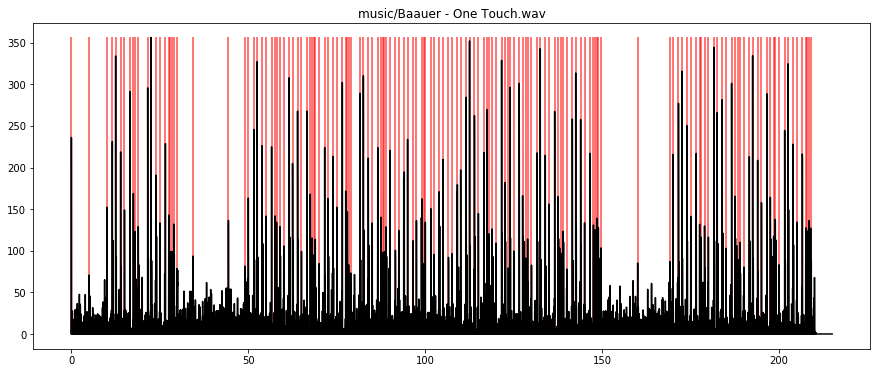
\includegraphics[scale=.6]{"src/pics/1.png"}
\par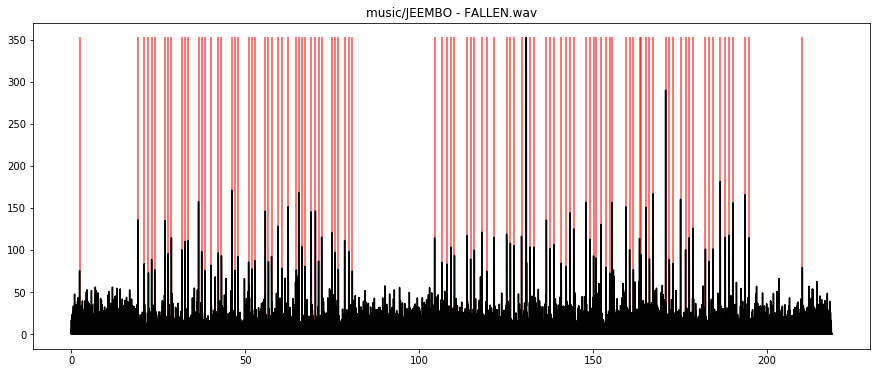
\includegraphics[scale=.6]{"src/pics/2.png"}
\par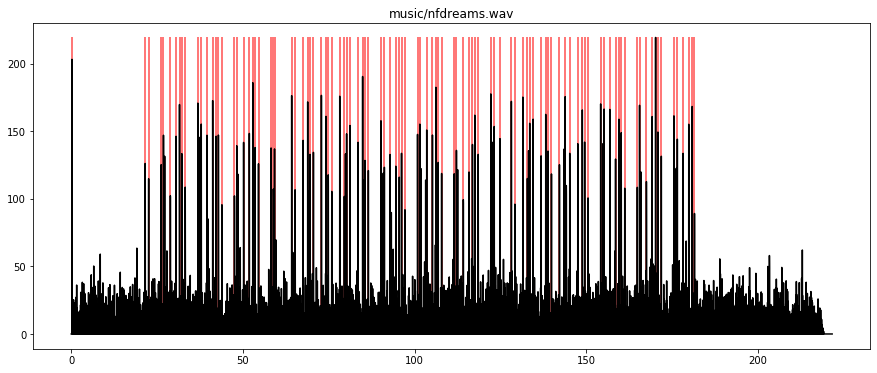
\includegraphics[scale=.6]{"src/pics/3.png"}

\par Более того, можно использовать ф-цию \verb|librosa.clicks| чтобы сгенерировать клики в местах удара, т.о. совместив клики с песней можно прослушать песню определив, правильно ли определяются удары (все сказанное есть в jupyter notebook в директории \verb|client/sandbox/|)
\section*{Ссылка на GitHub}
\href{https://github.com/Kipparis/Colored-Music}{github.com/Kipparis/Colored-Music}
\pagebreak
